% Options for packages loaded elsewhere
\PassOptionsToPackage{unicode}{hyperref}
\PassOptionsToPackage{hyphens}{url}
%
\documentclass[
]{article}
\usepackage{amsmath,amssymb}
\usepackage{lmodern}
\usepackage{ifxetex,ifluatex}
\ifnum 0\ifxetex 1\fi\ifluatex 1\fi=0 % if pdftex
  \usepackage[T1]{fontenc}
  \usepackage[utf8]{inputenc}
  \usepackage{textcomp} % provide euro and other symbols
\else % if luatex or xetex
  \usepackage{unicode-math}
  \defaultfontfeatures{Scale=MatchLowercase}
  \defaultfontfeatures[\rmfamily]{Ligatures=TeX,Scale=1}
\fi
% Use upquote if available, for straight quotes in verbatim environments
\IfFileExists{upquote.sty}{\usepackage{upquote}}{}
\IfFileExists{microtype.sty}{% use microtype if available
  \usepackage[]{microtype}
  \UseMicrotypeSet[protrusion]{basicmath} % disable protrusion for tt fonts
}{}
\makeatletter
\@ifundefined{KOMAClassName}{% if non-KOMA class
  \IfFileExists{parskip.sty}{%
    \usepackage{parskip}
  }{% else
    \setlength{\parindent}{0pt}
    \setlength{\parskip}{6pt plus 2pt minus 1pt}}
}{% if KOMA class
  \KOMAoptions{parskip=half}}
\makeatother
\usepackage{xcolor}
\IfFileExists{xurl.sty}{\usepackage{xurl}}{} % add URL line breaks if available
\IfFileExists{bookmark.sty}{\usepackage{bookmark}}{\usepackage{hyperref}}
\hypersetup{
  pdftitle={Code Metrics for the full system in R},
  pdfauthor={Aarón Blanco Álvarez},
  hidelinks,
  pdfcreator={LaTeX via pandoc}}
\urlstyle{same} % disable monospaced font for URLs
\usepackage[margin=1in]{geometry}
\usepackage{color}
\usepackage{fancyvrb}
\newcommand{\VerbBar}{|}
\newcommand{\VERB}{\Verb[commandchars=\\\{\}]}
\DefineVerbatimEnvironment{Highlighting}{Verbatim}{commandchars=\\\{\}}
% Add ',fontsize=\small' for more characters per line
\usepackage{framed}
\definecolor{shadecolor}{RGB}{248,248,248}
\newenvironment{Shaded}{\begin{snugshade}}{\end{snugshade}}
\newcommand{\AlertTok}[1]{\textcolor[rgb]{0.94,0.16,0.16}{#1}}
\newcommand{\AnnotationTok}[1]{\textcolor[rgb]{0.56,0.35,0.01}{\textbf{\textit{#1}}}}
\newcommand{\AttributeTok}[1]{\textcolor[rgb]{0.77,0.63,0.00}{#1}}
\newcommand{\BaseNTok}[1]{\textcolor[rgb]{0.00,0.00,0.81}{#1}}
\newcommand{\BuiltInTok}[1]{#1}
\newcommand{\CharTok}[1]{\textcolor[rgb]{0.31,0.60,0.02}{#1}}
\newcommand{\CommentTok}[1]{\textcolor[rgb]{0.56,0.35,0.01}{\textit{#1}}}
\newcommand{\CommentVarTok}[1]{\textcolor[rgb]{0.56,0.35,0.01}{\textbf{\textit{#1}}}}
\newcommand{\ConstantTok}[1]{\textcolor[rgb]{0.00,0.00,0.00}{#1}}
\newcommand{\ControlFlowTok}[1]{\textcolor[rgb]{0.13,0.29,0.53}{\textbf{#1}}}
\newcommand{\DataTypeTok}[1]{\textcolor[rgb]{0.13,0.29,0.53}{#1}}
\newcommand{\DecValTok}[1]{\textcolor[rgb]{0.00,0.00,0.81}{#1}}
\newcommand{\DocumentationTok}[1]{\textcolor[rgb]{0.56,0.35,0.01}{\textbf{\textit{#1}}}}
\newcommand{\ErrorTok}[1]{\textcolor[rgb]{0.64,0.00,0.00}{\textbf{#1}}}
\newcommand{\ExtensionTok}[1]{#1}
\newcommand{\FloatTok}[1]{\textcolor[rgb]{0.00,0.00,0.81}{#1}}
\newcommand{\FunctionTok}[1]{\textcolor[rgb]{0.00,0.00,0.00}{#1}}
\newcommand{\ImportTok}[1]{#1}
\newcommand{\InformationTok}[1]{\textcolor[rgb]{0.56,0.35,0.01}{\textbf{\textit{#1}}}}
\newcommand{\KeywordTok}[1]{\textcolor[rgb]{0.13,0.29,0.53}{\textbf{#1}}}
\newcommand{\NormalTok}[1]{#1}
\newcommand{\OperatorTok}[1]{\textcolor[rgb]{0.81,0.36,0.00}{\textbf{#1}}}
\newcommand{\OtherTok}[1]{\textcolor[rgb]{0.56,0.35,0.01}{#1}}
\newcommand{\PreprocessorTok}[1]{\textcolor[rgb]{0.56,0.35,0.01}{\textit{#1}}}
\newcommand{\RegionMarkerTok}[1]{#1}
\newcommand{\SpecialCharTok}[1]{\textcolor[rgb]{0.00,0.00,0.00}{#1}}
\newcommand{\SpecialStringTok}[1]{\textcolor[rgb]{0.31,0.60,0.02}{#1}}
\newcommand{\StringTok}[1]{\textcolor[rgb]{0.31,0.60,0.02}{#1}}
\newcommand{\VariableTok}[1]{\textcolor[rgb]{0.00,0.00,0.00}{#1}}
\newcommand{\VerbatimStringTok}[1]{\textcolor[rgb]{0.31,0.60,0.02}{#1}}
\newcommand{\WarningTok}[1]{\textcolor[rgb]{0.56,0.35,0.01}{\textbf{\textit{#1}}}}
\usepackage{graphicx}
\makeatletter
\def\maxwidth{\ifdim\Gin@nat@width>\linewidth\linewidth\else\Gin@nat@width\fi}
\def\maxheight{\ifdim\Gin@nat@height>\textheight\textheight\else\Gin@nat@height\fi}
\makeatother
% Scale images if necessary, so that they will not overflow the page
% margins by default, and it is still possible to overwrite the defaults
% using explicit options in \includegraphics[width, height, ...]{}
\setkeys{Gin}{width=\maxwidth,height=\maxheight,keepaspectratio}
% Set default figure placement to htbp
\makeatletter
\def\fps@figure{htbp}
\makeatother
\setlength{\emergencystretch}{3em} % prevent overfull lines
\providecommand{\tightlist}{%
  \setlength{\itemsep}{0pt}\setlength{\parskip}{0pt}}
\setcounter{secnumdepth}{-\maxdimen} % remove section numbering
\ifluatex
  \usepackage{selnolig}  % disable illegal ligatures
\fi

\title{Code Metrics for the full system in R}
\author{Aarón Blanco Álvarez}
\date{28/4/2021}

\begin{document}
\maketitle

\begin{center}\rule{0.5\linewidth}{0.5pt}\end{center}

\begin{figure}
\centering

\includegraphics{ual.jpg}
\caption{Logo de la UAL}
\end{figure}

\begin{center}\rule{0.5\linewidth}{0.5pt}\end{center}

\hypertarget{introduction}{%
\section{Introduction}\label{introduction}}

In this report we are going to discuss the evolution in the three
versions of Lucene. For this goal, we need tools to make the analysis
like R Studio, R, etc. With this approach, will get metrics of the
system in a clear way than other tools and also, R provide us the
possibility of make our own metrics.

\hypertarget{materials-and-methods}{%
\section{Materials and methods}\label{materials-and-methods}}

For our purpose, we need RStudio with R, the programming language
itself. Also, the data in csv from the execution of Sourcemeter.
Furthermore, we will install some packages to load csv among others.
Here is an example:

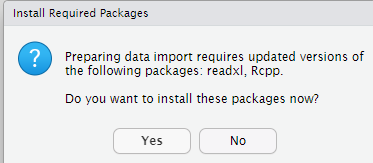
\includegraphics{EXCEL.png} \# Read xls

\begin{Shaded}
\begin{Highlighting}[]
\FunctionTok{library}\NormalTok{(readxl)}
\NormalTok{luc49\_Class }\OtherTok{\textless{}{-}} \FunctionTok{read\_excel}\NormalTok{(}\StringTok{"Excel/Lucene4.9.0/luc49{-}Class.xlsx"}\NormalTok{)}
\NormalTok{luc491\_Class }\OtherTok{\textless{}{-}} \FunctionTok{read\_excel}\NormalTok{(}\StringTok{"Excel/Lucene4.9.1/luc491{-}Class.xlsx"}\NormalTok{)}
\NormalTok{luc410\_Class }\OtherTok{\textless{}{-}} \FunctionTok{read\_excel}\NormalTok{(}\StringTok{"Excel/Lucene4.10/luc410{-}Class.xlsx"}\NormalTok{)}
\end{Highlighting}
\end{Shaded}

\hypertarget{system-metrics}{%
\section{System Metrics}\label{system-metrics}}

Let us start with the main metrics, after import the excel, we will use
R to read the excels.

\hypertarget{method-hiding-factor-mhf-}{%
\subsection{(Method Hiding Factor
--MHF-)}\label{method-hiding-factor-mhf-}}

This is the proportion of hiding methods. Firstly, we have to read the
excels, we can do that with the \textbf{read.csv} instruction, after
that, we can save the columns need it in two variables. In this case, NM
and NPM. The meaning of this two variables are \emph{number of methods}
and \emph{number of public methods}.

\begin{Shaded}
\begin{Highlighting}[]
\NormalTok{NM }\OtherTok{\textless{}{-}}\NormalTok{ luc49\_Class[[}\StringTok{"NM"}\NormalTok{]];}
\NormalTok{NPM }\OtherTok{\textless{}{-}}\NormalTok{ luc49\_Class[[}\StringTok{"NPM"}\NormalTok{]];}
\NormalTok{Privado4}\FloatTok{.9} \OtherTok{\textless{}{-}}\NormalTok{ (}\DecValTok{1}\SpecialCharTok{{-}}\NormalTok{(}\FunctionTok{sum}\NormalTok{(NPM)}\SpecialCharTok{/}\FunctionTok{sum}\NormalTok{(NM)));}
\FunctionTok{print}\NormalTok{(Privado4}\FloatTok{.9}\NormalTok{);}
\end{Highlighting}
\end{Shaded}

\begin{verbatim}
## [1] 0.1861779
\end{verbatim}

\begin{Shaded}
\begin{Highlighting}[]
\NormalTok{NM }\OtherTok{\textless{}{-}}\NormalTok{ luc491\_Class[[}\StringTok{"NM"}\NormalTok{]];}
\NormalTok{NPM }\OtherTok{\textless{}{-}}\NormalTok{ luc491\_Class[[}\StringTok{"NPM"}\NormalTok{]];}
\NormalTok{Privado4.}\FloatTok{9.1} \OtherTok{\textless{}{-}}\NormalTok{ (}\DecValTok{1}\SpecialCharTok{{-}}\NormalTok{(}\FunctionTok{sum}\NormalTok{(NPM)}\SpecialCharTok{/}\FunctionTok{sum}\NormalTok{(NM)));}
\FunctionTok{print}\NormalTok{(Privado4.}\FloatTok{9.1}\NormalTok{);}
\end{Highlighting}
\end{Shaded}

\begin{verbatim}
## [1] 0.1843877
\end{verbatim}

\begin{Shaded}
\begin{Highlighting}[]
\NormalTok{NM }\OtherTok{\textless{}{-}}\NormalTok{ luc410\_Class[[}\StringTok{"NM"}\NormalTok{]];}
\NormalTok{NPM }\OtherTok{\textless{}{-}}\NormalTok{ luc410\_Class[[}\StringTok{"NPM"}\NormalTok{]];}
\NormalTok{Privado4}\FloatTok{.1} \OtherTok{\textless{}{-}}\NormalTok{ (}\DecValTok{1}\SpecialCharTok{{-}}\NormalTok{(}\FunctionTok{sum}\NormalTok{(NPM)}\SpecialCharTok{/}\FunctionTok{sum}\NormalTok{(NM)));}
\FunctionTok{print}\NormalTok{(Privado4}\FloatTok{.1}\NormalTok{);}
\end{Highlighting}
\end{Shaded}

\begin{verbatim}
## [1] 0.18451
\end{verbatim}

As we can see, we can get private methods proportion if we make the
operation of divide number of public methods between all methods, then,
subtract to one. In theory, with each version, MHF is increasing, which
means that will be less bugs and technical debt, nevertheless, is very
small in this case.

\hypertarget{attribute-hiding-factor-ahf-}{%
\subsection{(Attribute Hiding Factor
--AHF-)}\label{attribute-hiding-factor-ahf-}}

This is the proportion of hiding attributes. In this metric, we can make
the same as before but in this case, changing the number of methods for
attributes. So, we are working here with the number of attributes and
NPA, public attributes. The formula is almost the same, but we are
working with that two columns.

\begin{Shaded}
\begin{Highlighting}[]
\NormalTok{NAtt }\OtherTok{\textless{}{-}}\NormalTok{ luc49\_Class[[}\StringTok{"NAtt"}\NormalTok{]];}
\NormalTok{NPA }\OtherTok{\textless{}{-}}\NormalTok{ luc49\_Class[[}\StringTok{"NPA"}\NormalTok{]];}
\NormalTok{APrivado }\OtherTok{\textless{}{-}} \DecValTok{1}\SpecialCharTok{{-}}\NormalTok{(}\FunctionTok{sum}\NormalTok{(NPA)}\SpecialCharTok{/}\FunctionTok{sum}\NormalTok{(NAtt));}
\FunctionTok{print}\NormalTok{(APrivado);}
\end{Highlighting}
\end{Shaded}

\begin{verbatim}
## [1] 0.5661251
\end{verbatim}

\begin{Shaded}
\begin{Highlighting}[]
\NormalTok{NAtt }\OtherTok{\textless{}{-}}\NormalTok{ luc491\_Class[[}\StringTok{"NAtt"}\NormalTok{]];}
\NormalTok{NPA }\OtherTok{\textless{}{-}}\NormalTok{ luc491\_Class[[}\StringTok{"NPA"}\NormalTok{]];}
\NormalTok{APrivado4\_9 }\OtherTok{\textless{}{-}} \DecValTok{1}\SpecialCharTok{{-}}\NormalTok{(}\FunctionTok{sum}\NormalTok{(NPA)}\SpecialCharTok{/}\FunctionTok{sum}\NormalTok{(NAtt));}
\FunctionTok{print}\NormalTok{(APrivado4\_9);}
\end{Highlighting}
\end{Shaded}

\begin{verbatim}
## [1] 0.5661843
\end{verbatim}

\begin{Shaded}
\begin{Highlighting}[]
\NormalTok{NAtt }\OtherTok{\textless{}{-}}\NormalTok{ luc410\_Class[[}\StringTok{"NAtt"}\NormalTok{]];}
\NormalTok{NPA }\OtherTok{\textless{}{-}}\NormalTok{ luc410\_Class[[}\StringTok{"NPA"}\NormalTok{]];}
\NormalTok{APrivado4\_1 }\OtherTok{\textless{}{-}}\NormalTok{ (}\DecValTok{1}\SpecialCharTok{{-}}\NormalTok{(}\FunctionTok{sum}\NormalTok{(NPA)}\SpecialCharTok{/}\FunctionTok{sum}\NormalTok{(NAtt)));}
\FunctionTok{print}\NormalTok{(APrivado4\_1);}
\end{Highlighting}
\end{Shaded}

\begin{verbatim}
## [1] 0.5661031
\end{verbatim}

Ideally, all attributes should be hidden, nevertheless, 56\% it is a
reasonable percentage. Anyways, we can see that in this case, there is a
little decrease in the results between versions, but the idea would be
increase the proportion of hidden attributes.

\hypertarget{method-inheritance-factor-mif-}{%
\subsection{(Method Inheritance Factor
--MIF-)}\label{method-inheritance-factor-mif-}}

Inheritance factor means the proportion of inherits methods. So, we can
calculate it subtracting the total number of methods with local public
methods. After that, we have to divide it from the total number of
methods.

\begin{Shaded}
\begin{Highlighting}[]
\NormalTok{NM }\OtherTok{\textless{}{-}}\NormalTok{ luc49\_Class[[}\StringTok{"NM"}\NormalTok{]];}
\NormalTok{NLM }\OtherTok{\textless{}{-}}\NormalTok{ luc49\_Class[[}\StringTok{"NLM"}\NormalTok{]];}
\NormalTok{HEREADOS }\OtherTok{\textless{}{-}}\NormalTok{ (NM }\SpecialCharTok{{-}}\NormalTok{ NLM);}
\NormalTok{MIF }\OtherTok{\textless{}{-}}\NormalTok{ (}\FunctionTok{sum}\NormalTok{(HEREADOS)}\SpecialCharTok{/}\FunctionTok{sum}\NormalTok{(NM));}
\FunctionTok{print}\NormalTok{(MIF);}
\end{Highlighting}
\end{Shaded}

\begin{verbatim}
## [1] 0.8437718
\end{verbatim}

\begin{Shaded}
\begin{Highlighting}[]
\NormalTok{NM }\OtherTok{\textless{}{-}}\NormalTok{ luc491\_Class[[}\StringTok{"NM"}\NormalTok{]];}
\NormalTok{NLM }\OtherTok{\textless{}{-}}\NormalTok{ luc491\_Class[[}\StringTok{"NLM"}\NormalTok{]];}
\NormalTok{HEREADOS }\OtherTok{\textless{}{-}}\NormalTok{ (NM }\SpecialCharTok{{-}}\NormalTok{ NLM);}
\NormalTok{MIF4.}\FloatTok{9.1} \OtherTok{\textless{}{-}}\NormalTok{ (}\FunctionTok{sum}\NormalTok{(HEREADOS)}\SpecialCharTok{/}\FunctionTok{sum}\NormalTok{(NM));}
\FunctionTok{print}\NormalTok{(MIF4.}\FloatTok{9.1}\NormalTok{);}
\end{Highlighting}
\end{Shaded}

\begin{verbatim}
## [1] 0.8452233
\end{verbatim}

\begin{Shaded}
\begin{Highlighting}[]
\NormalTok{NM }\OtherTok{\textless{}{-}}\NormalTok{ luc410\_Class[[}\StringTok{"NM"}\NormalTok{]];}
\NormalTok{NLM }\OtherTok{\textless{}{-}}\NormalTok{ luc410\_Class[[}\StringTok{"NLM"}\NormalTok{]];}
\NormalTok{HEREADOS }\OtherTok{\textless{}{-}}\NormalTok{ (NM }\SpecialCharTok{{-}}\NormalTok{ NLM);}
\NormalTok{MIF4}\FloatTok{.1} \OtherTok{\textless{}{-}}\NormalTok{ (}\FunctionTok{sum}\NormalTok{(HEREADOS)}\SpecialCharTok{/}\FunctionTok{sum}\NormalTok{(NM));}
\FunctionTok{print}\NormalTok{(MIF4}\FloatTok{.1}\NormalTok{);}
\end{Highlighting}
\end{Shaded}

\begin{verbatim}
## [1] 0.8453527
\end{verbatim}

In this case, we have a high percentage. This range should not be low
but also, not very high, this indicates either superfluous inheritance
or too wide member scopes. In this example, the proportion is
increasing, nevertheless, there is not a major change.

\hypertarget{attribute-inheritance-factor-aif-}{%
\subsection{(Attribute Inheritance Factor
--AIF-)}\label{attribute-inheritance-factor-aif-}}

This metric is similar to MIF but in this case, we are talking about the
attributes.

\begin{Shaded}
\begin{Highlighting}[]
\NormalTok{NAtt }\OtherTok{\textless{}{-}}\NormalTok{ luc49\_Class[[}\StringTok{"NAtt"}\NormalTok{]];}
\NormalTok{NLA }\OtherTok{\textless{}{-}}\NormalTok{ luc49\_Class[[}\StringTok{"NLA"}\NormalTok{]];}
\NormalTok{HEREADOS }\OtherTok{\textless{}{-}}\NormalTok{ (NAtt }\SpecialCharTok{{-}}\NormalTok{ NLA);}
\NormalTok{MIF }\OtherTok{\textless{}{-}}\NormalTok{ (}\FunctionTok{sum}\NormalTok{(HEREADOS)}\SpecialCharTok{/}\FunctionTok{sum}\NormalTok{(NAtt));}
\FunctionTok{print}\NormalTok{(MIF);}
\end{Highlighting}
\end{Shaded}

\begin{verbatim}
## [1] 0.8042234
\end{verbatim}

\begin{Shaded}
\begin{Highlighting}[]
\NormalTok{NAtt }\OtherTok{\textless{}{-}}\NormalTok{ luc491\_Class[[}\StringTok{"NAtt"}\NormalTok{]];}
\NormalTok{NLA }\OtherTok{\textless{}{-}}\NormalTok{ luc491\_Class[[}\StringTok{"NLA"}\NormalTok{]];}
\NormalTok{HEREADOS }\OtherTok{\textless{}{-}}\NormalTok{ (NAtt }\SpecialCharTok{{-}}\NormalTok{ NLA);}
\NormalTok{MIF4.}\FloatTok{9.1} \OtherTok{\textless{}{-}}\NormalTok{ (}\FunctionTok{sum}\NormalTok{(HEREADOS)}\SpecialCharTok{/}\FunctionTok{sum}\NormalTok{(NAtt));}
\FunctionTok{print}\NormalTok{(MIF4.}\FloatTok{9.1}\NormalTok{);}
\end{Highlighting}
\end{Shaded}

\begin{verbatim}
## [1] 0.8042521
\end{verbatim}

\begin{Shaded}
\begin{Highlighting}[]
\NormalTok{NAtt }\OtherTok{\textless{}{-}}\NormalTok{ luc410\_Class[[}\StringTok{"NAtt"}\NormalTok{]];}
\NormalTok{NLA }\OtherTok{\textless{}{-}}\NormalTok{ luc410\_Class[[}\StringTok{"NLA"}\NormalTok{]];}
\NormalTok{HEREADOS }\OtherTok{\textless{}{-}}\NormalTok{ (NAtt }\SpecialCharTok{{-}}\NormalTok{ NLA);}
\NormalTok{MIF4}\FloatTok{.1} \OtherTok{\textless{}{-}}\NormalTok{ (}\FunctionTok{sum}\NormalTok{(HEREADOS)}\SpecialCharTok{/}\FunctionTok{sum}\NormalTok{(NAtt));}
\FunctionTok{print}\NormalTok{(MIF4}\FloatTok{.1}\NormalTok{);}
\end{Highlighting}
\end{Shaded}

\begin{verbatim}
## [1] 0.8026854
\end{verbatim}

The results indicate that we may have a high rate of inherits
attributes. As in MIF metrics, both should be lower, this could be done
with the use of Interfaces instead of Inherits.

\hypertarget{polymorphism-factor-pf}{%
\subsection{Polymorphism Factor (PF)}\label{polymorphism-factor-pf}}

This metric was impossible to get since we have not got the number of
overrides methods.

\begin{Shaded}
\begin{Highlighting}[]
\CommentTok{\#The formula should be something like:}
\CommentTok{\# PF = overrides / sum for each class(new methods * descendants)}
\end{Highlighting}
\end{Shaded}

\hypertarget{coupling-factor-cf-}{%
\subsection{(Coupling Factor --CF-)}\label{coupling-factor-cf-}}

This metric indicates the coupling factor, which measures couplings
among classes. In other words, the communication between classes. This
formula use the column CBO, which means the total number of classes that
use other classes, furthermore, we have to use NOA, the number of
ancestors. To make the metric work, we need the number of total classes
too. We have that number getting any column and measure it with length.

\begin{Shaded}
\begin{Highlighting}[]
\NormalTok{CBO }\OtherTok{\textless{}{-}}\NormalTok{ luc49\_Class[[}\StringTok{"CBO"}\NormalTok{]];}
\NormalTok{NOA }\OtherTok{\textless{}{-}}\NormalTok{ luc49\_Class[[}\StringTok{"NOA"}\NormalTok{]];}
\NormalTok{numeroClases }\OtherTok{\textless{}{-}} \FunctionTok{length}\NormalTok{(luc49\_Class[[}\StringTok{"ID"}\NormalTok{]]);}
\NormalTok{NumR }\OtherTok{\textless{}{-}}\NormalTok{ CBO}\SpecialCharTok{{-}}\NormalTok{NOA;}
\NormalTok{CF }\OtherTok{\textless{}{-}}\NormalTok{ (numeroClases }\SpecialCharTok{{-}} \DecValTok{1}\NormalTok{)}\SpecialCharTok{/}\FunctionTok{sum}\NormalTok{(NumR);}
\FunctionTok{print}\NormalTok{(CF);}
\end{Highlighting}
\end{Shaded}

\begin{verbatim}
## [1] 0.192708
\end{verbatim}

\begin{Shaded}
\begin{Highlighting}[]
\NormalTok{CBO }\OtherTok{\textless{}{-}}\NormalTok{ luc491\_Class[[}\StringTok{"CBO"}\NormalTok{]];}
\NormalTok{NOA }\OtherTok{\textless{}{-}}\NormalTok{ luc491\_Class[[}\StringTok{"NOA"}\NormalTok{]];}
\NormalTok{numeroClases }\OtherTok{\textless{}{-}} \FunctionTok{length}\NormalTok{(luc491\_Class[[}\StringTok{"ID"}\NormalTok{]]);}
\NormalTok{NumR }\OtherTok{\textless{}{-}}\NormalTok{ CBO}\SpecialCharTok{{-}}\NormalTok{NOA;}
\NormalTok{CF }\OtherTok{\textless{}{-}}\NormalTok{ (numeroClases }\SpecialCharTok{{-}} \DecValTok{1}\NormalTok{)}\SpecialCharTok{/}\FunctionTok{sum}\NormalTok{(NumR);}
\FunctionTok{print}\NormalTok{(CF);}
\end{Highlighting}
\end{Shaded}

\begin{verbatim}
## [1] 0.1926064
\end{verbatim}

\begin{Shaded}
\begin{Highlighting}[]
\NormalTok{CBO }\OtherTok{\textless{}{-}}\NormalTok{ luc410\_Class[[}\StringTok{"CBO"}\NormalTok{]];}
\NormalTok{NOA }\OtherTok{\textless{}{-}}\NormalTok{ luc410\_Class[[}\StringTok{"NOA"}\NormalTok{]];}
\NormalTok{numeroClases }\OtherTok{\textless{}{-}} \FunctionTok{length}\NormalTok{(luc410\_Class[[}\StringTok{"ID"}\NormalTok{]]);}
\NormalTok{NumR }\OtherTok{\textless{}{-}}\NormalTok{ CBO}\SpecialCharTok{{-}}\NormalTok{NOA;}
\NormalTok{CF }\OtherTok{\textless{}{-}}\NormalTok{ (numeroClases }\SpecialCharTok{{-}} \DecValTok{1}\NormalTok{)}\SpecialCharTok{/}\FunctionTok{sum}\NormalTok{(NumR);}
\FunctionTok{print}\NormalTok{(CF);}
\end{Highlighting}
\end{Shaded}

\begin{verbatim}
## [1] 0.1914854
\end{verbatim}

As we can see, we have also no big differences, nevertheless, we can see
how the coupling factor is decreasing with every version.

\hypertarget{personal-metrics.}{%
\subsection{Personal metrics.}\label{personal-metrics.}}

\hypertarget{proportion-number-of-methods-for-total-lines-of-code-nmtlc.}{%
\section{Proportion Number of Methods for total lines of code
(NMTLC).}\label{proportion-number-of-methods-for-total-lines-of-code-nmtlc.}}

We can create a new metric using the proportion of number of methods
divide by lines of code. This could leads us to measure the complexity.

\begin{Shaded}
\begin{Highlighting}[]
\NormalTok{LOC1 }\OtherTok{\textless{}{-}}\NormalTok{ luc49\_Class[[}\StringTok{"LOC"}\NormalTok{]];}
\NormalTok{NM1 }\OtherTok{\textless{}{-}}\NormalTok{ luc49\_Class[[}\StringTok{"NM"}\NormalTok{]];}
\NormalTok{Total1 }\OtherTok{\textless{}{-}}\NormalTok{ (}\FunctionTok{sum}\NormalTok{(LOC1))}\SpecialCharTok{/}\FunctionTok{sum}\NormalTok{(NM1);}
\FunctionTok{print}\NormalTok{(Total1);}
\end{Highlighting}
\end{Shaded}

\begin{verbatim}
## [1] 3.043147
\end{verbatim}

\begin{Shaded}
\begin{Highlighting}[]
\NormalTok{LOC2 }\OtherTok{\textless{}{-}}\NormalTok{ luc491\_Class[[}\StringTok{"LOC"}\NormalTok{]];}
\NormalTok{NM2 }\OtherTok{\textless{}{-}}\NormalTok{ luc491\_Class[[}\StringTok{"NM"}\NormalTok{]];}
\NormalTok{Total2 }\OtherTok{\textless{}{-}}\NormalTok{ (}\FunctionTok{sum}\NormalTok{(LOC2))}\SpecialCharTok{/}\FunctionTok{sum}\NormalTok{(NM2);}
\FunctionTok{print}\NormalTok{(Total2);}
\end{Highlighting}
\end{Shaded}

\begin{verbatim}
## [1] 3.015236
\end{verbatim}

\begin{Shaded}
\begin{Highlighting}[]
\NormalTok{LOC3 }\OtherTok{\textless{}{-}}\NormalTok{ luc410\_Class[[}\StringTok{"LOC"}\NormalTok{]];}
\NormalTok{NM3 }\OtherTok{\textless{}{-}}\NormalTok{ luc410\_Class[[}\StringTok{"NM"}\NormalTok{]];}
\NormalTok{Total3 }\OtherTok{\textless{}{-}}\NormalTok{ (}\FunctionTok{sum}\NormalTok{(LOC3))}\SpecialCharTok{/}\FunctionTok{sum}\NormalTok{(NM3);}
\FunctionTok{print}\NormalTok{(Total3);}
\end{Highlighting}
\end{Shaded}

\begin{verbatim}
## [1] 2.986877
\end{verbatim}

\begin{Shaded}
\begin{Highlighting}[]
\NormalTok{media }\OtherTok{\textless{}{-}} \FunctionTok{c}\NormalTok{(Total1, Total2, Total3)}

\NormalTok{barMedia }\OtherTok{\textless{}{-}} \FunctionTok{barplot}\NormalTok{(media, }\AttributeTok{names =} \FunctionTok{c}\NormalTok{(}\StringTok{"version 4.9"}\NormalTok{, }\StringTok{"version 4.9.1"}\NormalTok{, }\StringTok{"version4.10"}\NormalTok{), }\AttributeTok{ylim =} \FunctionTok{c}\NormalTok{(}\DecValTok{0}\NormalTok{,}\FloatTok{3.5}\NormalTok{), }\AttributeTok{xlab =} \StringTok{"Versiones"}\NormalTok{, }\AttributeTok{main =} \StringTok{"NMTLC"}\NormalTok{, }\AttributeTok{col =} \FunctionTok{c}\NormalTok{(}\DecValTok{2}\NormalTok{,}\DecValTok{7}\NormalTok{,}\DecValTok{3}\NormalTok{))}
\FunctionTok{text}\NormalTok{(barMedia, media }\SpecialCharTok{{-}}\FloatTok{2.5}\NormalTok{, }\FunctionTok{paste}\NormalTok{(}\StringTok{"NMTLC= "}\NormalTok{, }\FunctionTok{format}\NormalTok{(}\FunctionTok{round}\NormalTok{(media, }\DecValTok{3}\NormalTok{), }\AttributeTok{nsmall =} \DecValTok{3}\NormalTok{), }\AttributeTok{sep=}\StringTok{""}\NormalTok{), }\AttributeTok{cex=}\DecValTok{0}\NormalTok{)}
\end{Highlighting}
\end{Shaded}

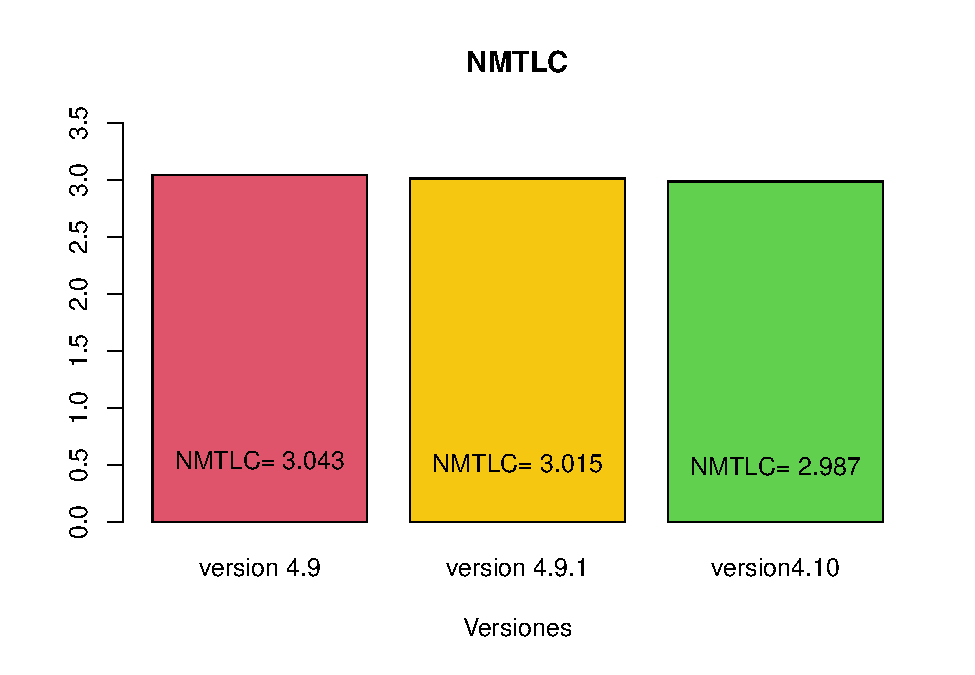
\includegraphics{report_files/figure-latex/unnamed-chunk-8-1.pdf}

In this case, the proportion is low, so we could think that in this
case, there is not a large complexity, nevertheless, this may not be the
best metric calculate the complexity, although is clearly that with
every version, the complexity is lower.

With this metric we can think that in some cases like more than 4,5
lines of code per method means that we will have high complexity. let us
review that.

\begin{Shaded}
\begin{Highlighting}[]
\FunctionTok{filter}\NormalTok{(LOC1[}\DecValTok{2}\NormalTok{]}\SpecialCharTok{/}\NormalTok{NM1[}\DecValTok{2}\NormalTok{] }\SpecialCharTok{\textgreater{}=} \DecValTok{4}\NormalTok{,}\DecValTok{5}\NormalTok{ );}
\end{Highlighting}
\end{Shaded}

\begin{verbatim}
## Time Series:
## Start = 1 
## End = 1 
## Frequency = 1 
## [1] 5
\end{verbatim}

\begin{Shaded}
\begin{Highlighting}[]
\FunctionTok{print}\NormalTok{(LOC1[}\DecValTok{2}\NormalTok{]);}
\end{Highlighting}
\end{Shaded}

\begin{verbatim}
## [1] 9
\end{verbatim}

\begin{Shaded}
\begin{Highlighting}[]
\FunctionTok{print}\NormalTok{(NM1[}\DecValTok{2}\NormalTok{]);}
\end{Highlighting}
\end{Shaded}

\begin{verbatim}
## [1] 2
\end{verbatim}

\begin{Shaded}
\begin{Highlighting}[]
\FunctionTok{print}\NormalTok{(LOC1[}\DecValTok{2}\NormalTok{]}\SpecialCharTok{/}\NormalTok{NM1[}\DecValTok{2}\NormalTok{]);}
\end{Highlighting}
\end{Shaded}

\begin{verbatim}
## [1] 4.5
\end{verbatim}

\begin{Shaded}
\begin{Highlighting}[]
\FunctionTok{filter}\NormalTok{(LOC1[}\DecValTok{6}\NormalTok{]}\SpecialCharTok{/}\NormalTok{NM1[}\DecValTok{6}\NormalTok{] }\SpecialCharTok{\textless{}=} \DecValTok{4}\NormalTok{,}\DecValTok{5}\NormalTok{ );}
\end{Highlighting}
\end{Shaded}

\begin{verbatim}
## Time Series:
## Start = 1 
## End = 1 
## Frequency = 1 
## [1] 5
\end{verbatim}

\begin{Shaded}
\begin{Highlighting}[]
\FunctionTok{print}\NormalTok{(LOC1[}\DecValTok{6}\NormalTok{]);}
\end{Highlighting}
\end{Shaded}

\begin{verbatim}
## [1] 53
\end{verbatim}

\begin{Shaded}
\begin{Highlighting}[]
\FunctionTok{print}\NormalTok{(NM1[}\DecValTok{6}\NormalTok{]);}
\end{Highlighting}
\end{Shaded}

\begin{verbatim}
## [1] 106
\end{verbatim}

\begin{Shaded}
\begin{Highlighting}[]
\FunctionTok{print}\NormalTok{(LOC1[}\DecValTok{6}\NormalTok{]}\SpecialCharTok{/}\NormalTok{NM1[}\DecValTok{6}\NormalTok{]);}
\end{Highlighting}
\end{Shaded}

\begin{verbatim}
## [1] 0.5
\end{verbatim}

In the example above, we can see two cases, for example, in the first
one, the proportion is low, this is because in the first row, we have
many methods, in the second case, we don't have methods, so the
proportion is lower than 4,5.

\hypertarget{attribute-mean}{%
\section{Attribute mean}\label{attribute-mean}}

This metric provide us with information about our classes, more
attributes could indicate low encapsulation, with leads us to a low
quality code. For example, if you are defining a class Person, and this
one have attribute like name, surname, email, street, city, number, etc,
one attribute like address could encapsulate all in other class instead
of have every attribute in class Person.

So, in this case, we have a way of check this.

\begin{Shaded}
\begin{Highlighting}[]
 \FunctionTok{library}\NormalTok{(dplyr)}
\end{Highlighting}
\end{Shaded}

\begin{verbatim}
## 
## Attaching package: 'dplyr'
\end{verbatim}

\begin{verbatim}
## The following objects are masked from 'package:stats':
## 
##     filter, lag
\end{verbatim}

\begin{verbatim}
## The following objects are masked from 'package:base':
## 
##     intersect, setdiff, setequal, union
\end{verbatim}

\begin{Shaded}
\begin{Highlighting}[]
\NormalTok{ luc49\_Class }\OtherTok{\textless{}{-}} \FunctionTok{filter}\NormalTok{(luc49\_Class, NAtt }\SpecialCharTok{\textgreater{}} \DecValTok{0}\NormalTok{)}
\NormalTok{ NAtt1NotEmpty }\OtherTok{\textless{}{-}}\NormalTok{ luc49\_Class[[}\StringTok{"NAtt"}\NormalTok{]];}
\NormalTok{ MediaNatt1 }\OtherTok{\textless{}{-}} \FunctionTok{mean}\NormalTok{(NAtt1NotEmpty)}

 \FunctionTok{print}\NormalTok{(MediaNatt1);}
\end{Highlighting}
\end{Shaded}

\begin{verbatim}
## [1] 15.26778
\end{verbatim}

\begin{Shaded}
\begin{Highlighting}[]
\NormalTok{ luc491\_Class }\OtherTok{\textless{}{-}} \FunctionTok{filter}\NormalTok{(luc491\_Class, NAtt }\SpecialCharTok{\textgreater{}} \DecValTok{0}\NormalTok{)}
\NormalTok{ NAtt2NotEmpty }\OtherTok{\textless{}{-}}\NormalTok{ luc491\_Class[[}\StringTok{"NAtt"}\NormalTok{]];}
\NormalTok{ MediaNatt2 }\OtherTok{\textless{}{-}} \FunctionTok{mean}\NormalTok{(NAtt2NotEmpty)}

 \FunctionTok{print}\NormalTok{(MediaNatt2);}
\end{Highlighting}
\end{Shaded}

\begin{verbatim}
## [1] 15.2671
\end{verbatim}

\begin{Shaded}
\begin{Highlighting}[]
\NormalTok{ luc410\_Class }\OtherTok{\textless{}{-}} \FunctionTok{filter}\NormalTok{(luc410\_Class, NAtt }\SpecialCharTok{\textgreater{}} \DecValTok{0}\NormalTok{)}
\NormalTok{ NAtt3NotEmpty }\OtherTok{\textless{}{-}}\NormalTok{ luc410\_Class[[}\StringTok{"NAtt"}\NormalTok{]];}
\NormalTok{ MediaNatt3 }\OtherTok{\textless{}{-}} \FunctionTok{mean}\NormalTok{(NAtt3NotEmpty)}
 \FunctionTok{print}\NormalTok{(MediaNatt3);}
\end{Highlighting}
\end{Shaded}

\begin{verbatim}
## [1] 15.35326
\end{verbatim}

\begin{Shaded}
\begin{Highlighting}[]
 \FunctionTok{boxplot}\NormalTok{(NAtt1NotEmpty,}
        \AttributeTok{main =} \StringTok{"Número de atributos"}\NormalTok{,}
        \AttributeTok{ylab =} \StringTok{"Atributos"}\NormalTok{,}
        \AttributeTok{col =} \StringTok{"red"}\NormalTok{,}
        \AttributeTok{border =} \StringTok{"purple"}\NormalTok{,}
        \AttributeTok{names =} \FunctionTok{c}\NormalTok{(}\StringTok{"Version 9.0"}\NormalTok{)}
        
\NormalTok{        )}
\end{Highlighting}
\end{Shaded}

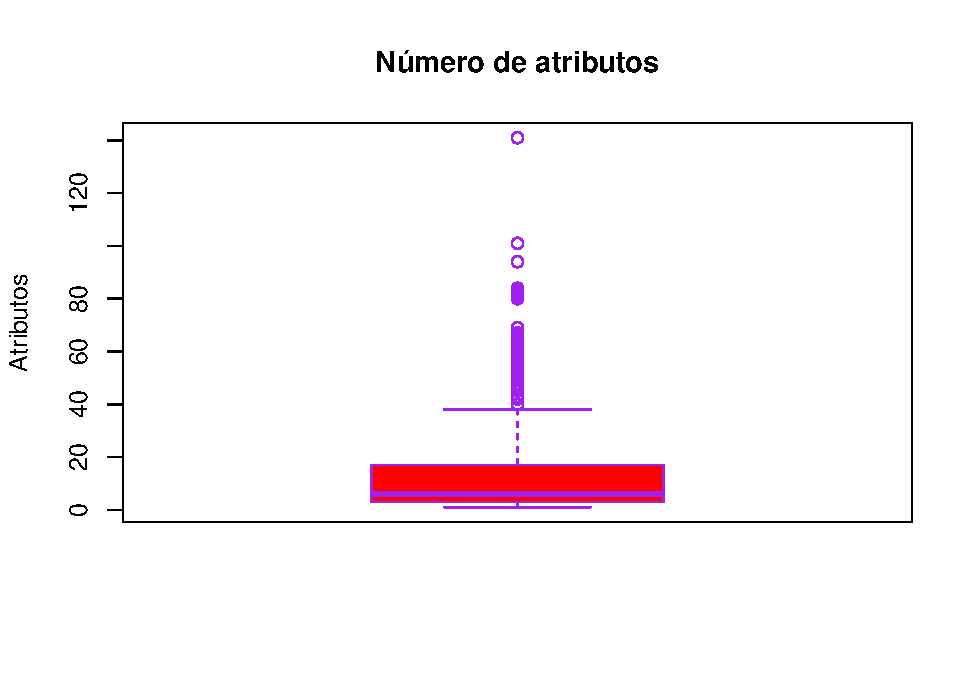
\includegraphics{report_files/figure-latex/unnamed-chunk-10-1.pdf}

\begin{Shaded}
\begin{Highlighting}[]
  \FunctionTok{boxplot}\NormalTok{(NAtt2NotEmpty,}
        \AttributeTok{main =} \StringTok{"Número de atributos"}\NormalTok{,}
        \AttributeTok{ylab =} \StringTok{"Atributos"}\NormalTok{,}
        \AttributeTok{col =} \StringTok{"green"}\NormalTok{,}
        \AttributeTok{border =} \StringTok{"orange"}\NormalTok{,}
        \AttributeTok{names =} \FunctionTok{c}\NormalTok{(}\StringTok{"Version 9.1"}\NormalTok{)}
        
\NormalTok{        )}
\end{Highlighting}
\end{Shaded}

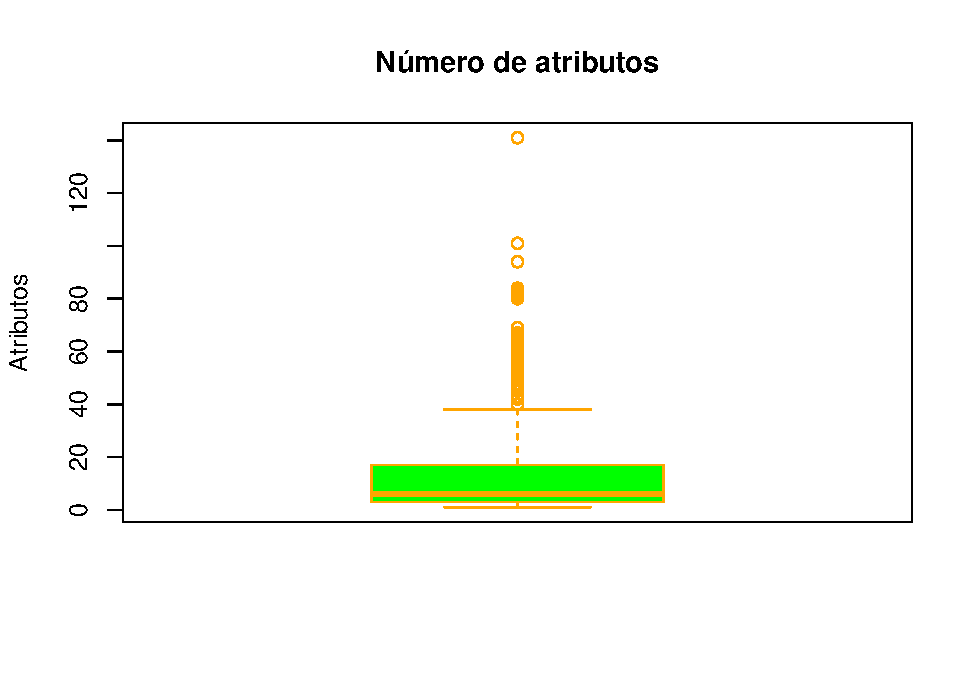
\includegraphics{report_files/figure-latex/unnamed-chunk-10-2.pdf}

\begin{Shaded}
\begin{Highlighting}[]
 \FunctionTok{boxplot}\NormalTok{(NAtt3NotEmpty,}
        \AttributeTok{main =} \StringTok{"Número de atributos"}\NormalTok{,}
        \AttributeTok{ylab =} \StringTok{"Atributos"}\NormalTok{,}
        \AttributeTok{col =} \StringTok{"blue"}\NormalTok{,}
        \AttributeTok{border =} \StringTok{"black"}\NormalTok{,}
        \AttributeTok{names =} \FunctionTok{c}\NormalTok{(}\StringTok{"Version 9.10"}\NormalTok{)}
        
\NormalTok{        )}
\end{Highlighting}
\end{Shaded}

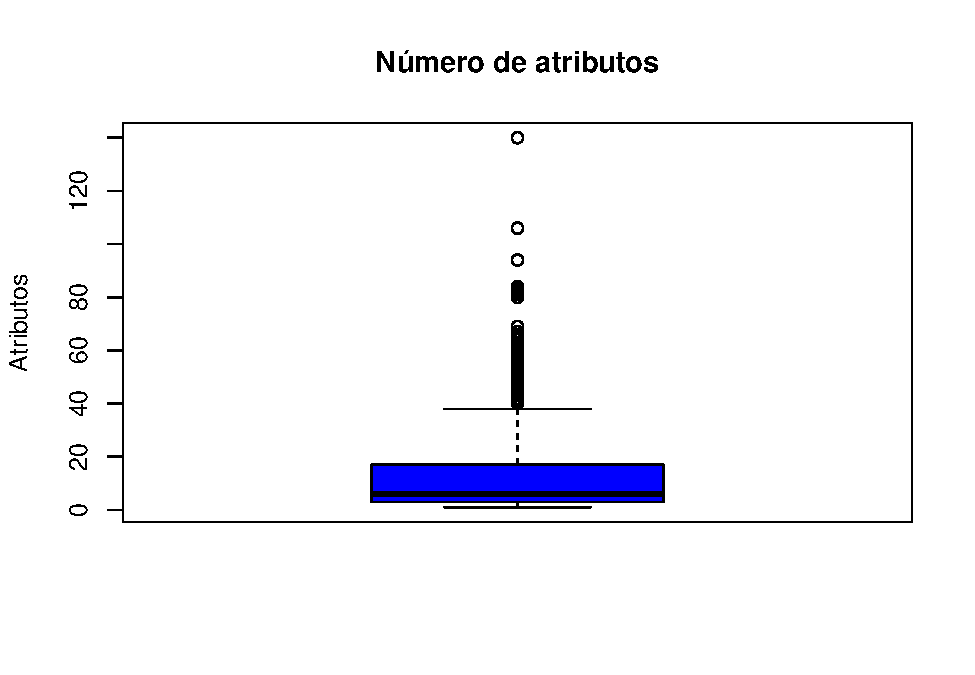
\includegraphics{report_files/figure-latex/unnamed-chunk-10-3.pdf}

What we have done it is a way of exclude classes with zero attribute and
then, calculate the mean. This provide us a way of take into account if
we are watching a complex class that may be encapsulate better. For
example, now that we know that the mean is of 15, we can see in the
graphs that some classes have up to 120, so, verify that should be
urgent. If we can verify classes, we only need to use a filter now that
we know the average.

\hypertarget{conclusions}{%
\section{Conclusions}\label{conclusions}}

To sum-up, we have observe the difference with every version, it is
seems clearly, that the previous version was better in most of the
cases, meaning that with the new releases, a few things could change,
leaving the code with less quality, nevertheless, this differences are
also minimal. Some of the indicators, show us the necessity of do
refactoring in the code, which can be a complex task in a big project
like Lucene, although, some things like the number of inherit attributes
should change in the future.

\end{document}
